\documentclass[11pt,pdftex]{article}

\usepackage{amsmath}
\usepackage{amsfonts}
\usepackage{graphicx}

\newcommand{\opal}{\textsc{OPAL}}
\newcommand{\opalt}{\textsc{OPAL-t }}
\newcommand{\opale}{\textsc{OPAL-e }}
\newcommand{\opalcycl}{\textsc{OPAL-cycl}}
\newcommand{\opalmap}{\textsc{OPAL-map }}
\newcommand{\opalenv}{\textsc{OPAL-envelop}}

\newcommand{\mad}{\textsc{mad }}
\newcommand{\madnine}{\textsc{mad9 }}
\newcommand{\madninep}{\textsc{mad9p }}
\newcommand{\madeight}{\textsc{mad8 }}

\newcommand{\classic}{\textsc{classic }}
\newcommand{\hfifepart}{\textsc{H5Part }}
\newcommand{\hfifefe}{\textsc{H5FED }}

\renewcommand{\epsilon}{\varepsilon} 
\renewcommand{\vec}[1]{{\bf #1}} 
\newcommand{\dt}[1]{\frac{\partial #1}{\partial t}}
\newcommand{\dtt}[1]{\frac{\partial^2 #1}{\partial t^2}}
\newcommand{\dtvec}[1]{\frac{\partial {\mathbf #1}}{\partial t}}
\newcommand{\dttvec}[1]{\frac{\partial^2 {\mathbf #1}}{\partial t^2}}
\newcommand{\rot}{\vec{\nabla} \wedge }
\renewcommand{\div}{\vec{\nabla} \cdot }

\def\vec#1{\mathbf{#1}}
\def\vecg#1{\boldsymbol{#1}}
\def\norm#1{\| #1 \|} 
\def\tr{^{\!\top}}

\def\curl{{\bf curl}\,}
\def\curlp{{\rm curl}_p\,}
\def\div{{\rm div}\,}
\def\grad{\nabla}
\def\gradp{\nabla_p}
\def\dotp#1#2{\langle#1,#2\rangle}
\def\eps{\varepsilon}

\newcommand{\mat}[1]{\ensuremath{\boldsymbol{#1}}}
\newcommand{\vect}[1]{\ensuremath{\mathbf{#1}}}
\newcommand{\iprod}[2]{\ensuremath{\langle#1,#2\rangle}}
\newcommand{\abs}[1]{\ensuremath{|#1|}}

\newcommand{\Nedelec}{N\'{e}d\'{e}lec}

\newcommand{\id}[1]{\structure{#1}}

\newcommand {\Co}{{\mathbb{C}}}
\newcommand {\Int}{{\mathbb{Z}}}
\newcommand {\Nat}{{\mathbb{N}}}
%
%
\newcommand {\Hcurl}{{H(\mathbf{curl};\Omega)}}
\newcommand {\Hocurl}{{H_0(\mathbf{curl};\Omega)}}
\newcommand {\Hdiv}{{H(\mathrm{div};\Omega)}}
\newcommand {\Hodiv}{{H_0(\mathbf{div};\Omega)}}
%
\renewcommand {\Re}{{\rm I \kern-2pt R}}
\newcommand{\vc}[1]{\mbox{\boldmath $#1$}}
\newcommand {\RM}[1]{\mathrm{#1}}



% A simple colored box inlined with the text
%  #1: color to use
%  #2: text to put
\newcommand{\INLINEBOX}[2]{%
   \begin{center}%
    \fcolorbox{#1!60!black}{#1}{%
      \addtolength{\linewidth}{-0.6cm}%  fixed value, works for normal article text
            \begin{minipage}{2\linewidth} #2 \end{minipage}%
  \begin{minipage}{\linewidth} #2 \end{minipage}%
    }%
   \end{center}\vspace{1pt}%
}

% A box at the margin containing the given text
\newcommand{\MARGINBOX}[1]{%
  \mbox{}%
  \marginpar%
   [\tiny\raggedleft\hspace{0pt}#1]%
   {\tiny\raggedright\hspace{0pt}#1}%
}

% mark specific elements: starred versions use inline boxes
\newcommand{\TODO}[2][]{\MARGINBOX{\textcolor{red!80!black}{\emph{ToDo (#1):}} #2}}
\WithSuffix\newcommand\TODO*[2][]{\INLINEBOX{red!20!white}{\emph{ToDo (#1):} #2}}

\newcommand{\FIXME}[2][]{\MARGINBOX{\textcolor{blue!80!black}{\emph{FixMe (#1):}} #2}}
\WithSuffix\newcommand\FIXME*[2][]{\INLINEBOX{blue!20!white}{\emph{FixMe (#1):} #2}}

\newcommand{\NOTE}[2][]{\MARGINBOX{\textcolor{green!80!black}{\emph{Note (#1):}} #2}}
\WithSuffix\newcommand\NOTE*[2][]{\INLINEBOX{green!20!white}{\emph{Note (#1):} #2}}

\newcommand{\DRAFT}[2][]{\MARGINBOX{\textcolor{blue!80!black}{\textsc{Draft (#1):}} #2}}
\WithSuffix\newcommand\DRAFT*[2][]{\INLINEBOX{blue!20!white}{\textsc{Draft (#1):} #2}}


\usepackage{url}
\usepackage{cite}
\usepackage{algorithm,algorithmic}
\usepackage{color}
\usepackage{bm}
\usepackage{a4}
\usepackage{url}
\usepackage{hyperref}
\usepackage{tikz}
\usepackage{pgflibraryshapes}  
\usetikzlibrary{arrows}
\usetikzlibrary{mindmap,trees}
\usepackage[overlay,absolute]{textpos}
\usepackage{pgfpages}


\TPGrid[4mm,25mm]{10}{5}

\textheight 9in \textwidth 6.5in
\topmargin -.2in \oddsidemargin 0cm

\newcommand{\gnuplotrot}{0.0}
\newcommand{\gnuplotscale}{0.5}
\newcommand{\minipagescale}{1.0}
\newcommand{\minipagescaleII}{.53}


%%%%%%%%%%%%%%%%%%%%%%%%%%%%%%%%%%%%%%%%%%%%%%%%%%%%%%%%%%%%%%%%%%%%%%%%%%%%%%5

\begin{document}

\setcounter{section}{1}
\section{Scientific Information on Project \\
  ``Scalable Parallel Adaptive Mesh Refinement \\
  with Application to ...''}

\begin{center}
  P. Arbenz, Chair of Computational Science, ETH, Zurich \\
  A. Adelmann, Large Research Facilities Division (GFA), Paul Scherrer
  Institut, Villigen
\end{center}

% \maketitle

% \vskip 5cm
% \noindent
% \emph{Key Words: AMR}  \newline

% \tableofcontents
% \setcounter{section}{0}
\section{General Part}
%
\begin{itemize}
\item
New Project

\item
Research Area: Numerical Analysis, Scientific Computing, CSE

\item
Duration: 24 Months, from April 1, 2011 - March 31, 2013.

\item
Beilagen: CV's/ Papers/ 

\noindent
List of Experts

\begin{itemize}
\item Prof. X.Y. Zzz, Applied Computer Science, California Institute of
  Technology, Pasadena, CA, USA 
\item Prof.\ Th.\ Schulthess, Director CSCS, Manno, Switzerland
\end{itemize}

\item
%
Requested Amount: 2 PostDocs at 60\% salary = %
                  2 $\times$ kCHF 95.4 + 100.3 for 2 years each = kCHF 391.4
%
\end{itemize}
%
% \setcounter{page}{0}
\newpage
%

\section{Summary}

TO BE WRITTEN.

\section{Scientific Part}

%%%%%%%%%%%%%%%%%%%%%%%%%%%%%%%%%%%%%%%%%%%%%%%%%%%%%%%%%%%%%%%%%%%%%%%%

\subsection{Introduction}
\label{sec:intro}

Large scale simulations by definition are simulations that deal with
large amounts of data.  In one of the applications that we target at in
this project, in the simulation of the Swiss Free Electron Laser
(SwissFEL), billions of particles are accelerated by an electric field
that is represented itself by billions of grid points in a mesh that
covers a domain of complicated shape.  The second application that we
are going to target in this project deals with the development of
Navier-Stokes / fluid-structure interaction / immersed interface
conditions.

Realistic grid-based simulations require fine mesh widths at locations
where quantities of interest vary rapidly\footnote{We use the terms
  `grid' and `mesh' interchangably.}.  Finite element approximations on
unstructured meshes very naturally can be arranged to fit the local
needs.  Unstructured meshes however are hard to adapt if the accuracy is
to be increased or in time dependent problems, where the location of the
action moves.  In any case, unstructured meshes require a substantial
overhead for storing information on the mesh topology.

In this project we will work with regular grids.  These are grids that
are obtained by applying some simple map to a rectangular grid.  Most of
the time the regular grid is rectangular itself.  Information on regular
grids is simple to store.  Furthermore, the regularity allows a fast
access to grid data and admits fast and memory efficient algorithms like
the FFT or geometric multigrid solvers.  This is the reason that most
simulations on highest end parallel computers are using regular grid
structures.

Also with regular grids adaptation is required to save memory space.
The straightforward approach to simply decrease grid spacings at
locations where high resolution is needed is not a good idea since the
regularity entails that the fine grid is extended to the boundary of the
computational domain.

There are two very different approaches that have emerged for grid
adaptation for regular grids.

\begin{enumerate}
  \begin{figure}[htb]
    \centering
    \includegraphics[width=0.75\textwidth]{figures/chombo-grids.png}  
    \caption{CHOMBO: 2D example illustrating proper nesting requirements
      for locally refined grids~\cite{chombo3.0}}
    \label{fig:chombo-grid}
  \end{figure}
\item In the 1980's Berger and Oliger~\cite{beol:84, beco:89} suggested
  to introduce a number of regular grids of varying grid spacings.  The
  coarsest grid embraces all finer grids.  Grids of equal grid spacing
  form a grid level.  Finer grids typically are (but need not be)
  aligned with the coordinate directions of coarser grids.  They cover
  only a fraction of the area of the coarser grid,
  cf.~Fig.~\ref{fig:chombo-grid}.
  %% 
  This approach has lead to a widly used software package called
  \texttt{CHOMBO}%
  \footnote{\url{https://seesar.lbl.gov/anag/chombo/}}.  The CHOMBO
  project is lead by Phil Colella of the Applied Numerical Algorithms
  Group (ANAG) at the Lawrence Berkeley National Laboratory.  In CHOMBO
  there exists a hierarchy of rectangular grids.  In each level of the
  hierarchy there is a set of (maybe unrelated) rectangular grids with a
  particular grid spacing.  Parallelism?

\item A second approch for adaptation in regular grids is based on
  octrees (quadtrees in two~space dimensions).  An octree (in graph
  theory) is a tree in which each internal node has exactly eight
  children.  Such trees arise naturally when subdividing a cube
  recursively into subcubes.
  %% 
  
  The root of the tree is a cube representing a coarsest grid that
  embraces the computational domain.  The subdivision proceeds to the
  desired depth.  Evidently such a tree can be (and will be in realistic
  problems) strongly unbalanced.  The tree can change in the course of a
  time-depending iteration process.  In a parallel implementation the
  distribution of the unbalanced tree is a crucial issue.  In DENDRO%
  \footnote{\url{http://www.cc.gatech.edu/csela/dendro/}}, the
  best-known software package that incorporates the octree approach, a
  space filling curve through the cubes corresponding to the nodes is
  used to that end.

\end{enumerate}

In this project we will address two applications that both `live' on
regular grids and the further development of both of them is hindered by
the large memory requirements of a single grid.

\begin{enumerate}
\item 
%%\textbf{\textsf{Space Charge Calculations at the \hipa\ Facility}}

  For the quantitative evaluation of the effects of \emph{space charge
    in the High Intensity Proton Accelerator} (\hipa) complex and the
  SwissFEL (one of the {\color{red}xxx} top priority projects in the ETH
  domain), an efficient three-dimensional particle tracking framwork
  Object Oriented Parallel Accelerator Library (\opal) \cite{opal:1} was
  developed.  Today \opal\ is the key tool to better understand the
  nonlinear space charge effects in the present and future particle
  accelerators at PSI and in several other research laboratories around
  the world.

  {\color{red}Here comes a characterization of the problem.}

 

  \begin{figure}[h]
    \begin{center}
      \includegraphics[width=1.0\linewidth]{./figures/xfel-gun}
      \caption{The SwissFEL electron gun under design, showing the primary beam in read and the 
      dark current electrons in green.}
      \label{fig:rre4ring}
    \end{center}
  \end{figure}



  {\color{red}FIXME: in that context motivate the need of AMR}

\item Here comes Giuseppe's contribution.
\end{enumerate}

{\color{red}\textbf{Project targets}}

\newpage


Some keywords: some of them have not been used so far.

A description of the application may follow here.

\medskip%
{\small

For long scientists try to reduce the amount of data without
compromising the accuracy of their results, i.e., \emph{to put the
  degrees of freedom where they are needed}.  In grid-based applications
this means the introduction of grids or meshes with varying grid
spacings.  We are aware of two software frameworks. 

time-dependence entails adaptation

In order to handle the 



Adaptive mesh refinement 

put the degrees of freedom where they are needed


Adaptation requires ``error indicators'' in order to determine where to
refine the mesh.



rectangular grids 

- rectangular subdomains, finite differences, finite volume method (CHOMBO)

- octree finite element method (DENDRO)


staggered grid

Problems to be solved: Poisson, Shallow-water, Navier-Stokes

Immersed interfaces and boundaries


\textbf{parallel implementation}: most codes are not implemented ``properly'' in
parallel.  Very often, the grid structure is stored redundantly.  In
large grids, this is a large amount of data.

OK for SMP

We identified two software frameworks that are in fact used 

What are the applications that we want to address.

C++ issues.

Experienced students needed to complete job in 2 years.

{\color{red}\textbf{High impact.}}

}

\subsection{Account of the state of research in the field}



\subsubsection{Chombo AMR Framework}

From B.V. Straalen \emph{et al.}~\cite{vslk:09}

AMR applications require a long-term sustained investment in software
infrastructure to create scalable solvers that are capable of utilizing
the full capabilities of the largest available HPC platforms. We have
created a framework for implementing scalable parallel AMR calculations
called Chombo [4] that provides an environment for rapidly assembling
portable, high-performance AMR applications for a broad variety of
scientific disciplines.

Chombo is a fully instrumented C++ library. There are a set of timer
macros that can be used to time functions or sections of code. These
timers attempt to use native instructions on the target architecture in
order to minimize the overhead of collecting detailed performance
data. In the case of the Cray XT, Chombo measures elapsed time using the
rdtsc x86 assembly instruction.  This returns a 64-bit unsigned integer
representing the number of clock cycles since last processor reset. On
the AMD Opteron processor this instruction takes, on average, 13 cycles
to execute, and for a 2.6GHz clock provides a 0.385 nanosecond timing
resolution.  The timers collect information which is summarized and
output at the end of a run for each processor.  The output of the Chombo
timing infrastructure is similar in format to the GNU profiler (gprof)
output but only instrumented functions and sections of code are
reported.  This information is then post-processed to produce various
statistics, e.g., mean/min/max times, standard deviations, and
correlations.  Additional analysis was performed using the

\subsubsection{Dendro  AMR Framework}

Current version: Dendro-3.0.1 of May 10, 2010.%
\footnote{\url{http://www.cc.gatech.edu/csela/dendro/}}
%%
Dendro was initially developed at the Computational science and
engineering laboratory (CSELa) at the University of Pennsylvania. It is
currently maintained by the Computational science and engineering
laboratory (CSELa) at the Georgia Institute of Technology.  The
principal investigator of the Dendro project is George Biros (Georgia
Institute of Technology, Atlanta GA, USA).

Dendro is a suite of parallel algorithms for the discretization and
solution of partial differential equations that require discretization
of second-order elliptic operators on rectangular grids~\cite{ssad:07,
  sasl:08, sabi:10, ssal:09}.  Dendro builds a hierarchy of ever smaller
cubes.  A cube can be (dynamically) subdivided in eight subcubes.  By
recursion, an octree structure is obtained.  Dendro supports trilinear
finite element discretizations on the subcubes.  The division of cubes
can, e.g., be based on error estimators.  There is a global restriction
on the way the partitioning of cubes can proceed: a so-called 2:1
balancing is enforced that limits the ratio of the edge lengths of
neighbored cells by 2:1.  
%%
\begin{figure}[h]
  \centering
  \includegraphics[width=0.65\textwidth]{figures/quadtree.png}  
  \caption{Dendro 2:1 balancing of a quadtree in two
    dimensions~\cite{sasl:08}}
  \label{fig:dendro}
\end{figure}
%%
The procedure is visualized in Fig.~\ref{fig:dendro} for the equivalent
2-dimensional situation.  In Fig.~\ref{fig:dendro}(b) a square is
displayed that has been refined three times.  Fig.~\ref{fig:dendro}(a)
displays the corresponding quadtree.  Since the the edge length of
square $h$ is four times the edge length of squares $c$ and $e$, square
$h$ id subdivided, with the result given in Fig.~\ref{fig:dendro}(c).
Of course, this procedure can in the worst case extend over the whole
domain.  However, it enhances the stability of a potential multigrid
solver.  It also limits he number of possible stencils in stencil-based
applications like PDE discratizations with finite-difference or
finite-volume methods.

Dendro works matrix free.  Matrix-vector multiplications are done in an
element-by-element fashion.  The system matrix as well as
prolongator/restrictor matrices in a multigrid solver are never built.

Dendro is free software, distributed under the terms of the GNU General
Public License.  It uses the following libraries: the Portable,
Extensible Toolkit for Scientific Computation (PETSc), the Message
Passing Interface (MPI), and the C++ Standard Template Library (STL).

Dendro has been used in various applications, mostly in connection with
problems from (bio-) mechanics.

Dendro has been used successfully on up to 12'000 processors for an
application in linear elasticity.  [{\color{red}References are missing
  here.}  Contacted George B. to get some.]

\subsubsection{Other software}

\begin{itemize}
\item The framework \textbf{Peano}%
  \footnote{\url{http://www5.in.tum.de/peano/}}%
  has been developed at the Institut f\"ur Informatik at TU
  Munich~\cite{mmnw:09, bumw:06, hakz:08}.  It is based on Peano's space
  filling curve.  Therefore, in the recursive refinement a cube is
  subdivided not in~8 but in 27~subcubes.  The approach is
  `cache-oblivious' on computers with a hierarchical memory arrangement.
  After an initial phase in the computation the data can be accessed
  with almost no cache misses.  The authors of Peano report cache hit
  rates above 99\%~\cite{hakz:08} in various applications, e.g., the
  Poisson equation, Navier-Stokes equation, and fluid-structure
  interaction.  Parallel computations have been executed on small
  clusters with less than~100 processors~\cite{mmnw:09}.  We have
  confirmed Peano's amazing cache efficiency in an application from
  elasticity~\cite{sche:10}.  The performance in the Peano framework
  originates in the storage of the data in a number of caches.  In
  3D~elasticity 27~stacks are employed.  During the computation the data
  is scattered in various memory locations and hierarchies.  Therefore,
  an initial phase is needed to get the data where it should be during
  the actual computation.  (This is in fact just a traversal of the
  space-filling curve.)  At the end of the computation the data has to
  be gather for further usage.  The framework is quite monolithic.  It
  is (almost) not possible to access single data items.

  If other software is used in the computation that expects data in the
  usual layout the scatter/gather procedure will have to be called
  often.  This will degrade the performance.

\item The \textbf{libMesh} library provides a framework for the
  numerical simulation of partial differential equations using arbitrary
  unstructured discretizations on serial and parallel platforms%
  \footnote{\url{http://libmesh.sourceforge.net/}}.  It has been (and
  still is) developed primarily at the University of Texas at Austin in
  the CFDLab.

  \texttt{libmesh} provides support for parallel adaptive mesh refinement
  and coarsening for finite element computations on irregular meshes.
  It uses PETSc and SLEPc for solving linear systems and eigenvalue
  problems.

  Unfortunately, in \texttt{libmesh} the grid information is replicated
  on all processors, such that it does not scale to a larger number of
  processors~\cite{kpsc:06}.  It does not support regular grids.

\item \textbf{RAMSES} was developed at the CEA in Saclay to study large
  scale structure and galaxy formation%
  \footnote{\url{http://irfu.cea.fr/Projets/Site_ramses/RAMSES.html}}.
  It is used in cosmologic simulations like galaxy formation and
  magneto-hydrodynamics.  It is written in Fortran~90.  MPI is used for
  the interprocessor communication.  AMR is implemented tree-based like
  in DENDRO.  

  The code is mainly used in astrophysics.  We know of efficient solves
  of the Poisson equation on a $2048^3$ grid on $2048$ processors.

\item \textbf{ALUgrid} provides an adaptive, load-balanced, and
  unstructured grid library%
  \footnote{\url{http://www.mathematik.uni-freiburg.de/IAM/Research/alugrid/}}.
  It is developed at the Applied Mathematics Department in
  Freiburg/Germany.  ALUGrid provides both hexahedral and tetrahedral
  grids.  There is an interface to the DUNE library~\cite{bdko:06}.

  The software is not used for large scale computing.  The ALUGrid
  webpage makes the impression that the software is not further
  developed, which usually means limited user support.
  
\end{itemize}




\subsection{Research plan}
\label{sec:research_plan}

\subsection{Account of the state of research in the field}


\subsubsection{Chair of Computational Science}

Extensive experience with the parallel solution of large numerical
problems is gathered at the Chair of Computational Science.  Based on
lectures of the PI and of Prof.~W.~Petersen (ETHZ) an ``Introduction to
Parallel Computing'' has been published recently by Oxford University
Press~\cite{pear:04}.  In recent years we were mainly concerned with
finite element simulations.  The collaboration with the group at the
Paul Scherrer Institut (PSI) and with the ETH Integrated Systems
Laboratory on accelerator cavities and lasers lead to a number of
papers, see e.g.~\cite{arga:01, arge:04, abgh:04, adai:10}.  These
simulations combined electromagnetics, accelerator physics and large
scale parallel computing.  Recent work concerns the partitioning of very
large finite element meshes on thousands of processors. This is a
crucial issue already for regular, block-structured cartesian grids
considered in the present project but even more so for irregular,
unstructured ones.  We have compared a number of approaches.  It turned
out that Recursive Coordinate Bisection (RCB)~\cite{debk:04} is much
more stable than the better known ParMETIS~\cite{metis}.

In a collaboration with the Institute of Biomechanics a fully parallel
and scalable code to solve the linear elasticity problem on the
complicated domains induced by human bones.  All portions of this code,
i.e., data distribution, matrix assembly, generation of the multigrid
preconditioner, solution, and I/O, are scalable to at least a 1000
processors~\cite{almm:06, almm:07, bcaf:10, wmvf:10}.  We have
investigated smoothed aggregation algebraic multigrid preconditioners in
eigensolvers for structural analysis~\cite{ahlt:05} as well.

Work of other groups at the Chair of Computational Science is on
multiscale modelling and simulation, high performance computing and
bioinspired optimization.  Expertise in programming Cell coprocessors
and in particular GPU's is available.  In~\cite{rbhk:09} an adaptive
wavelet-based solver has been designed and implemented on the ETH
cluster Brutus as well as on GPU's.






\subsubsection{Large Research Facilities Division (GFA), Paul Scherrer Institut}

\noindent Dr.~Adelmann has established and is leading the AMAS (Accelerator Modeling and Advanced Simulations) group, part of the Large Research Facilities (GFA) division
of the Paul Scherrer Institut (PSI).
%%
AMAS bridges the gap between qualitative and quantitative modeling by combining and extending
the latest developments in: (i) accelerator physics, (ii) numerical modeling and
(iii) high performance computing.
%%
At present 2 fte's, one post doc and $5$ PhD. students pursue their research in the field of self-consistent modeling
of particle accelerators, coherent synchrotron radiation modeling,
computation of electromagnetic eigenmodes in lossy cavities, precise modeling of the \hipa\ facility
and large-scale optimization accelerators. Four out of the 5 PhD. students in AMAS are supervised by Dr.~Adelmann.

Research at AMAS in the past have focused on two aspects: space-charge dominated beam transport in large structures \cite{adelmann2002, adelmann04-1,stingelin2005,geus:02} and electromagnetic modeling in the frequency domain (based on a time-harmonic ansatz for Maxwell�s equations) in large and complicated structures \cite{arge:04,abgh:06}.

Our focus at present is to enter into a regime of modeling that can be best described as a transition from  {\bf qualitative} to {\bf quantitative} modeling of large and complicated particle accelerator structures \cite{adelmann04-1} .\ 

We highlight three areas of research, relevant to this proposal: Eigenmode Calculations and Space Charge Calculations in the \hipa\ Facility.

\noindent \textbf{\textsf{Eigenmode Calculation}}

The first few eigenfrequencies of the PSI COMET cyclotron could be computed to high precision with the in-house developed time harmonic Maxwell solver 
FemaXX \cite{geus:02,arge:04}. The large (1.4 million degrees of freedom) and complex mesh is depicted in Figure \ref{fig:xt3cometfemaxx}, and in addition the parallel speedup during an eigenmode calculation of PSI's COMET cavities.

\begin{figure}[h]
\begin{minipage}[b]{\minipagescale\textwidth}
\includegraphics[angle=\gnuplotrot,scale=1.0]{./figures/Comet.pdf}
\includegraphics[angle=\gnuplotrot,scale=0.6]{./figures/xt3_comet1.pdf}
\end{minipage}
\caption{FemaXX mesh of PSI's COMET cyclotron (left) and  speedup  (right)}
\label{fig:xt3cometfemaxx}
\end{figure}
Table \ref{tab:cometmeas} shows the excellent agreement between the calculated and measured eigenfrequencies from PSI's Comet cyclotron. The number of significant figures in Table \ref{tab:cometmeas}  is determined by the physical boundary conditions of the tuning system and the accuracy of the measurement process. For the presented system a resolution of 10 kHz is absolutely sufficient.

\begin{table}[h]\footnotesize
\caption{Comparison between mode measurements from  PSI's Comet cyclotron and the calculated modes}
\begin{center}  
\begin{tabular}{lccc} 
\hline 
& Measurements [MHz]  & FemaXX \cite{geus:02}  \\
\hline
 Mode 1 (push/pull)	& 73.18	& 73.18   \\
Mode 2	&73.41	&73.44 \\
Mode 3 (pull/pull) &	73.64	&73.69 \\
Mode 4 &	92.71&	92.46 \\
\hline
\end{tabular}
\label{tab:cometmeas}
\end{center}
\end{table}

{\color{red}FIXME: a few words on paralleization and the potential for AMR.}


\noindent \textbf{\textsf{Space Charge Calculations at the \hipa\ Facility}}

For the quantitative evaluation of the effects of space charge in the high intensity proton accelerator complex and the SwissFEL (one of the xxx top priority projects in the ETH domain), an efficient three-dimensional particle tracking framwork Object Oriented Parallel Accelerator Library (\opal) \cite{opal:1} was developed. Today \opal is the key tool to better understand the nonlinear space charge effects in the present and future particle accelerators at PSI and in several other laboratories around the world.
In Figure \ref{fig:xt3opal}, the parallel scalability of the code is shown, which is absolutely essential for solving multi-scale problems, e.g.\ to track several millions of particles along kilometers of beam path in the cyclotrons and beam lines.  The data has been computed on the Cray massive parallel computer of the Swiss National Supercomputing Centre (CSCS) in Manno in the framework of the  PSI-Horizon collaboration \cite{horpsi}. 
 \begin{figure}[h]
    \begin{center}
      \includegraphics[angle=\gnuplotrot,scale=0.5]{./figures/drift2c1.pdf}
    \end{center}
    \caption{The parallel efficiency of the \opal\ kernel (strong scaling) is shown together with the number of particles pushed per time interval. A uniform mesh of the size $M=1024^3$ and 3d domain decomposition was used.}
    \label{fig:xt3opal}
  \end{figure}

Presently, we study different operation scenarios of the PSI Ring Cyclotron in the course of the planned high power upgrade and validate the physical and numerical mode with experiments. In Figure \ref{fig:rre4ring}
the beam intensity of the 8 last turns in the PSI Ring Cyclotron is compared with calculations. A remarkably good agreement of the turn patterns is observed and demonstrates the feasibility of precise beam dynamics
simulations on a scale necessary  for this research project. A particle matter interaction mode combined with full 3D space charge is also available, which is an indispensable tool for all future high intensity machines. 
\begin{figure}[h]
\begin{center}
\includegraphics[width=1.0\linewidth]{./figures/rre4v0108log}
\caption{Comparison of measured density profiles of the last 8 turns of the PSI Ring Cyclotron with \opal simulations (to be published \cite{bi:1}), showing a remarkable good agreement.}
\label{fig:rre4ring}
\end{center}
\end{figure}

{\color{red}FIXME: in that context motivate the need of AMR}

\noindent \textbf{\textsf{The Parallel Block Structured Framework \ippl}}

 \ippl (Independent Parallel Particle Layer) is an object-oriented framework for particle based applications in computational science 
requiring high-performance parallel computers. One of \ippl 's most attractive features is its high performance on both single-processor and distributed-memory multicomputers machines. 
\ippl  is a library of C++ classes designed to represent common abstractions in applications where {\em particles, fields} and operators like {\em FFT's} are needed.

Application programmers use and derive from these classes, which present a data-parallel programming interface at the highest abstraction layer.

Lower, to the user (programmer) hidden implementation layers encapsulate distribution and communication of data among processors. The supported platforms are: Linux based Beowulf clusters, Cray XT4/5, SGI Ultrix, IBM Blue Gene/L and Blue Gene/P.

The main goals of the \ippl  framework includes:
\begin{itemize}
    \item Portability across serial, distributed, and parallel architectures with no change to source code
    \item Development of reusable, cross-problem-domain components to enable rapid application development
    \item High efficiency for kernels and components relevant to scientific simulation
    \item Framework design and development driven by applications from a diverse set of scientific problem domains
    \item Shorter time from problem inception to working parallel simulations 
\end{itemize}

 \begin{figure}[h]
\begin{center}
 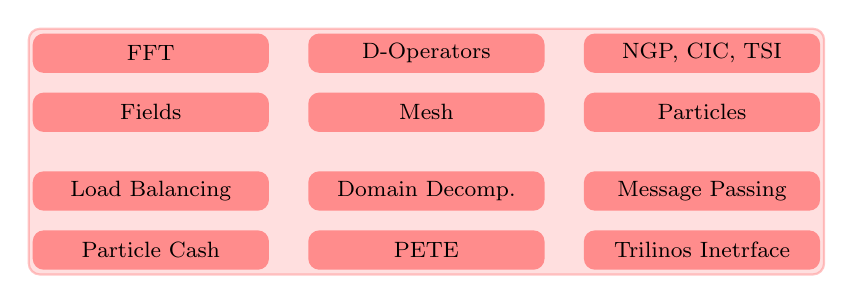
\begin{tikzpicture}[scale=1.0, transform shape]
    \footnotesize
      \begin{scope}[shape=rectangle,rounded corners,minimum width=3.0cm,minimum height=0.5cm,fill=yellow,text centered]
      \draw[rounded corners, draw=red!45, thick, fill=red!25, opacity=0.5, text centered] (-1.55, -0.69) rectangle (8.55,-3.81) 
                node[black, thick, anchor=center, opacity=1.0, font=\Large] at (3.5, -2.25) { };
       \node[fill= red!45] (q_00) at (0,-1) {FFT};
       \node[fill= red!45] (q_01) at (3.5,-1) {D-Operators};
       \node[fill= red!45] (q_02) at (7,-1) {NGP, CIC, TSI};
       \node[fill= red!45] (q_10) at (0,-1.75) {Fields};
       \node[fill= red!45] (q_11) at (3.5,-1.75) {Mesh};
       \node[fill= red!45] (q_12) at (7,-1.75) {Particles};
       \node[fill=red!45] (q_20) at (0,-2.75) {Load Balancing};
       \node[fill=red!45] (q_21) at (3.5,-2.75) {Domain Decomp.};
       \node[fill=red!45] (q_22) at (7,-2.75) {Message Passing};
       \node[fill=red!45] (q_20) at (0,-3.5) {Particle Cash};
       \node[fill=red!45] (q_21) at (3.5,-3.5) {PETE};
       \node[fill=red!45] (q_22) at (7,-3.5) {Trilinos Inetrface};
      \end{scope}
 \end{tikzpicture}
\end{center}
\caption{Architecture of \ippl}
\label{fig:ippl}
\end{figure}

{\color{red}FIXME: \opal is based on \ippl}
{\color{red}FIXME: show scaling of \ippl}

\noindent \textbf{\textsf{Summary Status of Research w.r.t this Proposal}}

The examples shown are good illustrations reflecting the strategy to closely connect theory and practical application in the developed methods and codes. In the past we have successfully developed methods and tools to simulate large and complicated accelerator structures. 

In the current research proposal numerical methods and accelerator modeling techniques developed in AMAS are indispensable because it provides the necessary level of detail in key areas such
as
\begin{itemize}
\item precise  3D beam dynamics modeling including loss predictions
\item large scale electromagnetic modeling capabilities for the resonator design.
\end{itemize}








%%%%%%%%%%%%%%%%%%%%%%%%%%%%%%%%%%%%%%%%%%%%%%%%%%%%%%%%%%%%%%%%%%%%%%%

\subsection{Detailed research plan}

\subsection*{Scientific and technical description}


\subsection{Timetable, milestones and deliverables}

The project is planned to last 3 years.  The various phases are
summarized in the following table.
%%
\begin{center}
  \begin{tabular}{|c|c|l|}
    \hline
    Phase & Duration & Work \\  \hline
    1 & 6 months &  Initial skill adaptation training \\
    2 & 12 months & Make \textsf{femaxx} a complex symmetric solver \\
    3 & 3 months & Extend for quadratic eigenvalue problem \\
    4 & 9 months & Extend for nonlinear eigenvalue problem \\
    5 & 6 months & Write thesis and wrap up \\  \hline
  \end{tabular}
\end{center}

%%%%%%%%%%%%%%%%%%%%%%%%%%%%%%%%%%%%%%%%%%%%%%%%%%%%%%%%%%%%%%%%%%%%%%%

\subsection{Significance of the planned research to the scientific
  community and to eventual potential users}
\label{sec:sign}

%%%%%%%%%%%%%%%%%%%%%%%%%%%%%%%%%%%%%%%%%%%%%%%%%%%%%%%%%%%%%%%%%%%%%%%

\subsection{Significance with respect to scientific, commercial, and
  other application areas}
\label{sec:sign2}

%\nocite{hens:05,cale:05,gbgk:05,vslk:09}
{\small
  \bibliography{amr,citation-aa}
  \bibliographystyle{plain}
}

\end{document}


% \newpage
% \subsection{Description of the Research}\label{sec:resdescr}
% \setcounter{subsection}{-1}
% \input{motivationandbackground.tex}
% \input{stateofart.tex}
% \input{stateownres.tex}
% \input{planofres.tex}
% \input{timetable.tex}
% \input{significance.tex}
% \input{cooperation.tex}
% \input{refhp2c.tex}
\end{document}
